%
% Chapter 3 - Results
%
\chapter{Results}

This chapter shows what has been achieved and developed to this date.\\

As previously written in the project's roadmap, this project has already a working relational database
and a HTTP server, developed with postgreSQL and with kotlin and spring mvc, respectively. The group also
managed to achieve, by this date as planned, its first working plaform client - the android mobile application, developed
with kotlin. This last one, it is still a prototype, so it lacks some features that will be completed during the next weeks.

\section{Relational database}

As a result of multiples redesigns, here is the database's final conceptual model.

\begin{figure}[H]    
    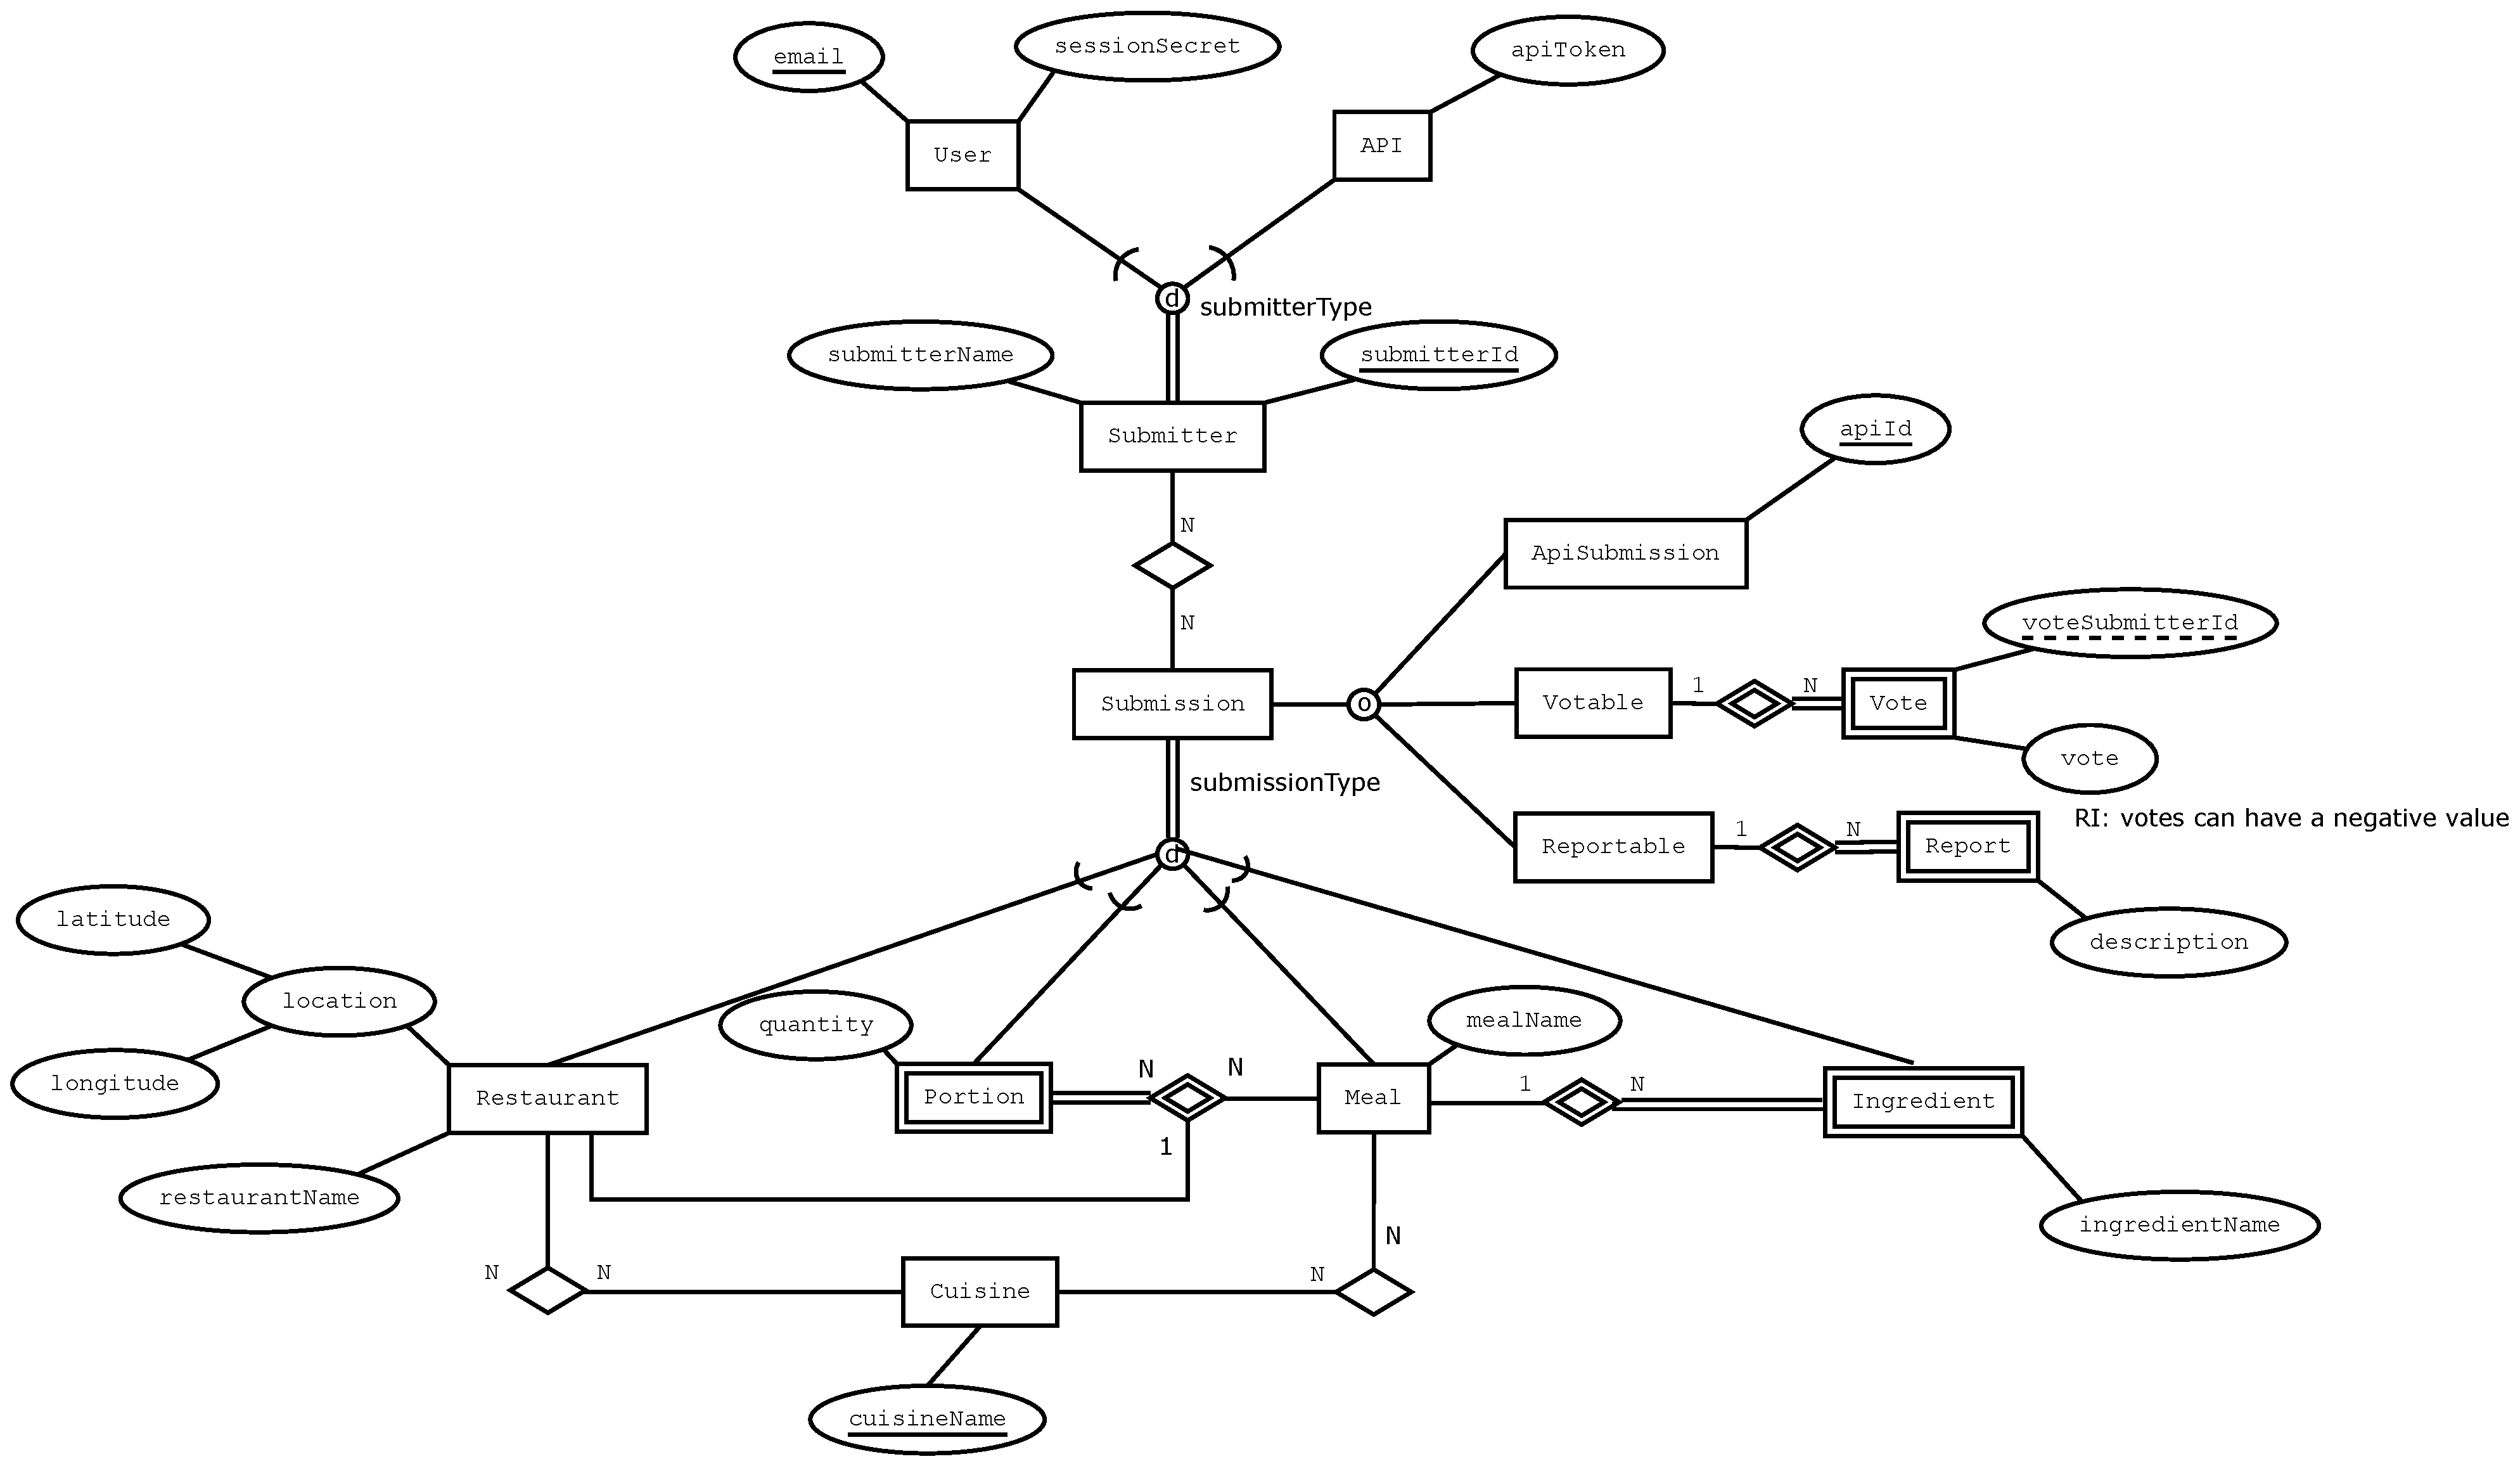
\includegraphics[scale=0.25]{_figures/Nutr.io_Database_Diagram.eps}
    \caption{Database conceptual model}
\end{figure}

\newpage
The database's relational model is present inside this report's appendix.\\

In the relational model there are tables which are not specified in the conceptual model previously presented,
those tables are a product from associations between entities, which will, not only facilitate the construction of the access queries,
as provide useful data to the HTTP server's endpoints.\\

The best feature of this redesigned model is that the database can filter the user submissions from the API submissions. This is very
useful, because when the user tries to associate a meal, that does not exist in the database, to a restaurant, that is already registered
in the database, the system will have search for that meal in an external API. When the meal is found, it will be inserted in the database
as an API submission, because the data came from an external API.\\

However if another user inserts this previously inserted meal to another registered restaurant, it will insert as an user's submission, because
the data already existed in the database and the user just built the association between this specific meal and the specific restaurant.\\

This algorithm, which resembles memory pointers, provides a high scalability to the database and, cooperatively with the database normalization, lowers the memory.

\section{HTTP server}

\section{Android application}